\documentclass[../main.tex]{subfiles}

\begin{document} %%%%%%%%%%%%%%%%%%%%%%%%%%%%%%%%%%%%%%%%%%%%%%%%%%%%%%%%%%%%
\section{Guía de ejercicios} 
    \subsection{Guía 1}
        \begin{exercise} 
            Una pequeña empresa de productos químicos debe consumir más de 40 $M^3$/mes de un determinado alcohol, debido a que ha firmado un contrato con la municipalidad de la zona (este alcohol es producido allí mismo). En compensación recibe beneficios impositivos. 
            
            Produce dos tipos de fertilizantes: A y B. En la tabla siguiente se da la información básica:
            \begin{table}[ht]
                \centering
                \begin{tabular}{l|l|l|}
                \cline{2-3}
                                                &  \textbf{Producto A} & \textbf{Producto B} \\ \hline
                \multicolumn{1}{|l|}{\textbf{Consumo de alcohol}} & 3 M³/unidad & 2/3 M³/unidad \\ \hline
                \multicolumn{1}{|l|}{\textbf{Consumo de ciclohexano}} & 1 tn/unidad & 2 tn/unidad \\ \hline
                \end{tabular}
                \caption{Tabla de datos}
            \end{table}

            \textbf{Disponibilidad de ciclohexano:} 20 tn. por mes.\\

            Con estas restricciones, y sabiendo que la contribución marginal es 1.200 \$/u para el producto A y 400 \$/u para el producto B, ¿cuál es el plan óptimo de producción?.\\

            \textbf{Solución:}
            \begin{enumerate}
                \item Objetivo del problema: Maximizar la contribución marginal total.
                \item Definir variables de decisión:
                    \begin{equation}
                        \begin{split}
                            x_1 &= \text{unidades producidas de fertilizante A [unidad/mes]} \\
                            x_2 &= \text{unidades producidas de fertilizante B [unidad/mes]} \\
                        \end{split}
                    \end{equation}
                \item Función objetivo (maximizar contribución marginal):
                    \begin{equation}
                        \max Z = 1200 \cdot x_1 + 400 \cdot x_2
                    \end{equation}
                \item Restricciones:
                    \begin{equation}
                        \begin{aligned}
                            3 \cdot x_1 + \frac{2}{3} \cdot x_2 &\geq 40 && \text{(Restricción de consumo de alcohol)} \\
                            x_1 + 2 \cdot x_2 &\leq 20 && \text{(Restricción de consumo de ciclohexano)}\\
                            x_1, x_2 & \geq 0 && \text{(No se pueden producir cantidades negativas de productos)}\\
                        \end{aligned}
                    \end{equation}


            \end{enumerate}

        \end{exercise}

        \begin{exercise}
            Hay tres máquinas disponibles para la producción de dos productos. Cada uno de ellos requiere los tiempos de proceso que se indican en la tabla siguiente (expresados en horas/unidad).
            \begin{table}[ht]
                \centering
                \begin{tabular}{|c|c|c|c|}
                \hline
                \textbf{Producto} & \textbf{Máq. A} & \textbf{Máq. B} & \textbf{Máq. C} \\ \hline
                \textbf{1} &    2      &     3     &    4      \\ \hline
                \textbf{2} &    4      &     2     &    2      \\ \hline
                \textbf{Disponibilidad (hs/mes)} &    80     &    60     &   100     \\ \hline
                \end{tabular}
                \caption{Tabla de datos}
            \end{table}

            El esquema del proceso productivo es el siguiente:
            \begin{itemize}
                \item Ambos productos deben pasar sucesivamente por las tres máquinas (en el orden “A→B→C”) para quedar totalmente terminados. Una máquina puede procesar un solo producto por vez.
                \item El precio de venta de 1 es de 60 \$/u y el de 2 es de 50 \$/u. Se planea la operación para el mes que viene.
            \end{itemize}

            ¿Cuál es el uso óptimo de estos recursos frente al objetivo de maximizar las ganancias?.\\

            \textbf{Solución:}
            \begin{enumerate}
                \item Objetivo del problema: Maximizar las ganancias.
                \item Definir variables:
                    \begin{equation}
                        \begin{split}
                            x_1 &= \text{unidades producidas de producto 1 [unidad/mes]} \\
                            x_2 &= \text{unidades producidas de producto 2 [unidad/mes]} \\
                        \end{split}
                    \end{equation}
                \item Función objetivo (maximizar ganancias):
                    \begin{equation}
                        \max Z = 60 \cdot x_1 + 50 \cdot x_2
                    \end{equation}
                \item Restricciones:
                    \begin{equation}
                        \begin{aligned}
                            2 \cdot x_1 + 4 \cdot x_2 &\leq 80 && \text{(Restricción de disponibilidad de máquina A)} \\
                            3 \cdot x_1 + 2 \cdot x_2 &\leq 60 && \text{(Restricción de disponibilidad de máquina B)}\\
                            4 \cdot x_1 + 2 \cdot x_2 &\leq 100 && \text{(Restricción de disponibilidad de máquina C)}\\
                            x_1, x_2 & \geq 0 && \text{(No se pueden producir cantidades negativas de productos)}\\
                        \end{aligned}
                    \end{equation}
                \item Representación gráfica:
                    \begin{figure}[ht]
                        \centering
                        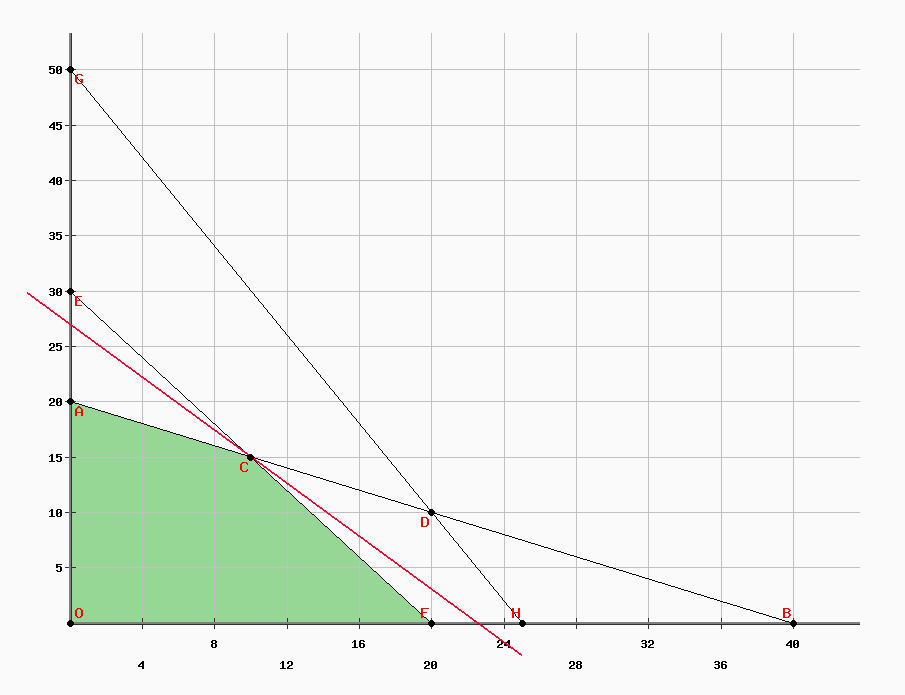
\includegraphics[width=0.9\textwidth]{./images/guia/1-2_ejercicio.png}
                        \caption{Representación gráfica del problema}
                    \end{figure}

                    Observando el gráfico, se puede ver que el punto óptimo es el punto $C(10,15)$, con un valor de $Z = 1350$.

                    \newpage
                    
                \item Obtención algebraicamente de la solución:
                    Tenemos que usar variables de holgura o slack variables para poder expresar las restricciones de igualdad como restricciones de desigualdad. Para ello, definimos las variables de holgura $s_1$, $s_2$ y $s_3$:
                    \begin{equation}
                        \begin{split}
                            s_1 &= \text{variable de holgura de la restricción de disponibilidad de máquina A} \\
                            s_2 &= \text{variable de holgura de la restricción de disponibilidad de máquina B} \\
                            s_3 &= \text{variable de holgura de la restricción de disponibilidad de máquina C} \\
                        \end{split}
                    \end{equation}
                    Con estas variables, podemos expresar las restricciones de igualdad como restricciones de desigualdad:
                    \begin{equation}
                        \begin{aligned}
                            2 \cdot x_1 + 4 \cdot x_2 + s_1 &= 80 && \text{(Restricción de disponibilidad de máquina A)} \\
                            3 \cdot x_1 + 2 \cdot x_2 + s_2 &= 60 && \text{(Restricción de disponibilidad de máquina B)}\\
                            4 \cdot x_1 + 2 \cdot x_2 + s_3 &= 100 && \text{(Restricción de disponibilidad de máquina C)}\\
                            x_1, x_2, s_1, s_2, s_3 & \geq 0 && \text{(No se pueden producir cantidades negativas de productos)}\\
                        \end{aligned}
                    \end{equation}



                    
            \end{enumerate}

        \end{exercise}

\end{document}  %%%%%%%%%%%%%%%%%%%%%%%%%%%%%%%%%%%%%%%%%%%%%%%%%%%%%%%%%%%%%
